%======================================================================
% GMI-04 Fibrovane prostory [PK 20261007].pdf
%======================================================================
\section{Fibrované prostory}
\strana{GMI-04a-1}

\begin{itemize}[nosep]
  \item Fibrované prostory (bandly)
  \item Vektorové bandly
  \item Trivializace a věta o rekonstrukci
  \item Netriviální bandly (příklady)
\end{itemize}

%----------------------------------------------------------------------
\newpage
\strana{GMI-04a-2}
\subsection{Fibrované prostory}

\begin{definice}[fibrovaný prostor (bandl)]
$\mathbb{E}M$ je \kw{fibrovaný prostor} se stand.\ fibrem $\mathbb{E}$ $\equiv$
\begin{itemize}[nosep]
  \item[] $\mathbb{E}M$ je dif.\ varieta \hfill -- \kw{totální prostor}, \kw{bandl}
  \item[] $M$ je dif.\ varieta \hfill -- \kw{podkladový} [base] \kw{prostor}
  \item[] $\mathbb{E}$ prostor s nějakou str.\ \hfill -- \kw{standardní vlákno} [fiber]
  \item[] $\pi:\mathbb{E}M\to M$ \quad projekce dávající fibraci
  \item[] $\mathbb{E}_xM = \pi^{-1}x$ \quad \kw{vlákno} [fiber] nad $x\in M$
  \item[] $\mathbb{E}_xM \cong \mathbb{E}$ \quad izomorfismus respektující strukturu standardního fibru
  \item[] \kw{lokální trivialita} $\mathbb{E}M$ -- restrikce na \uv{malou} oblast $U$ je triviální \\
          $\forall x\in M\ \exists$ okolí $U\subset M$, $x\in U$ tak, že $\mathbb{E}U$ je difeomorfní s $\mathbb{E}\times U$ \\
          difeomorfismus respektuje projekce a na fibrech dává izomorfismus $\mathbb{E}_xU\cong\mathbb{E}$
\end{itemize}
\end{definice}

\begin{vysvetleni}[Co je fibrovaný prostor]
Fibrovaný prostor (bandl) je \uv{rodina} kopií standardního vlákna $\mathbb{E}$, jedna kopie $\mathbb{E}_xM$ nad každým bodem $x\in M$,
slepená dohromady hladce. Značení $\mathbb{E}M$ čti \uv{bandl objektů typu $\mathbb{E}$ nad $M$}; $\mathbb{E}U\equiv\pi^{-1}(U)$ je jeho část nad $U\subset M$.
Klíčová je \emph{lokální trivialita}: nad malou oblastí $U$ vypadá bandl jako přímý součin $U\times\mathbb{E}$ (tj.\ \uv{bod báze $+$ hodnota ve vlákně}),
globálně ale může být \uv{zkroucený} (Möbiův pásek, Kleinova láhev, Hopfova fibrace -- viz dále).
Isomorfismus $\mathbb{E}_xM\cong\mathbb{E}$ přitom \emph{není kanonický} -- závisí na zvolené trivializaci.
Viz Krtouš, odd.~2.4 (kde se prostor polí s hodnotami v $\mathbb{E}_xM$ značí $\mathrm{Sect}\,\mathbb{E}M$).
\end{vysvetleni}

\begin{definice}[řezy fibrovaného prostoru]
\[
  \phi: M\to\mathbb{E}M \qquad x\mapsto\phi(x)\in\mathbb{E}_xM
\]
tj.\ \quad $\vzorec{\pi\circ\phi = \mathrm{id}}$
\end{definice}

tečný a kotečný bandly jsou vekt.\ fibr.\ prostory \\
\quad $\mathcal{T}M$ je prostor řezů $\mathbb{T}M$ \\
\quad $\mathcal{T}^*M$ je prostor řezů $\mathbb{T}^*M$

tečný a kotečný prostor je svázán s $M$ více než obecný fibrovaný prostor nad $M$

\begin{vysvetleni}[Řezy = pole]
Řez je \uv{pole}: v každém bodě $x$ vybereme jeden prvek vlákna nad $x$; podmínka $\pi\circ\phi=\mathrm{id}$ říká právě to, že $\phi(x)$ leží nad $x$.
Vektorové pole je tedy řez tečného bandlu, $\mathcal{T}M = \mathrm{Sect}\,\mathbb{T}M$, 1-forma řez kotečného bandlu (Krtouš, odd.~2.4).
\uv{Svázanost} tečného bandlu s $M$: $\mathbb{T}M$ je určen samotnou varietou -- jeho přechodová zobrazení jsou Jacobiho matice
$\partial x^i_{(\alpha)}/\partial x^j_{(\beta)}$ přechodů mezi mapami a každý difeomorfismus $M$ se přirozeně zvedá na $\mathbb{T}M$ (tlačení vpřed).
Obecný bandl nad $M$ takovou vazbu na souřadnice nemá (např.\ vnitřní prostor kalibračního pole).
\end{vysvetleni}

%----------------------------------------------------------------------
\newpage
\strana{GMI-04a-3}
\subsection{Vektorové fibrované bundly}

\begin{definice}[vektorový bandl]
$M$ varieta, $\mathbb{A}$ vekt.\ prostor \\
$\mathbb{A}M$ je \kw{vektorový bandl} nad $M$ se standardním fibrem $\mathbb{A}$ $\equiv$
\begin{itemize}[nosep]
  \item[] $\mathbb{A}M$ je dif.\ varieta
  \item[] $\pi:\mathbb{A}M\to M$ \quad diferencovatelná projekce
  \item[] $\mathbb{A}M$ lokálně triviální, tj.
  \[
    \forall x\in M\ \exists\, U\subset M \text{ okolí } x \qquad
    \pi^{-1}(U)\cong U\times\mathbb{A} \quad\text{tak, že}\quad
    \underbrace{\pi^{-1}y}_{\mathbb{A}_yM}\ \underset{\substack{\uparrow\\ \text{lineární zobr.}}}{\cong}\ y\times\mathbb{A}
  \]
  \item[] $\mathbb{A}_xM$ je fibr nad $x\in M$ \quad $\equiv$ \quad $\mathbb{A}_xM = \pi^{-1}x$
\end{itemize}
\end{definice}

\begin{definice}[řez vektorového bandlu]
$\mathbb{A}M$ vektorový bandl nad $M$ \\
$a$ je \kw{řez} $\mathbb{A}M$ $\equiv$
\[
  a: M\to\mathbb{A}M \quad\text{(diferencovatelné)}, \qquad \pi\circ a = \mathrm{id}
\]
$\mathrm{Sect}\,\mathbb{A}M$ $\equiv$ prostor všech řezů $\mathbb{A}M$
\end{definice}

\begin{vysvetleni}[Vektorový bandl a jeho řezy]
U vektorového bandlu má každé vlákno $\mathbb{A}_xM$ strukturu vektorového prostoru a lokální trivializace je na vláknech \emph{lineární}.
Díky tomu lze řezy sčítat a násobit funkcemi bod po bodu: $(a+b)(x)=a(x)+b(x)$, $(fa)(x)=f(x)\,a(x)$,
takže $\mathrm{Sect}\,\mathbb{A}M$ je modul nad okruhem hladkých funkcí $\mathcal{F}M$ (viz GMI-04b).
Vždy existuje \emph{nulový řez} $a(x)=0\in\mathbb{A}_xM$; netrivialita bandlu se projeví až tím, že nemusí existovat řez, který je všude nenulový.
\end{vysvetleni}

\begin{definice}[tenzorový bandl]
$\mathbb{A}M$ vekt.\ bandl nad $M$ se stand.\ fibrem $\mathbb{A}$ \\
$\mathbb{A}^k_lM$ tenz.\ bandl nad $M$ vygenerovaný $\mathbb{A}M$ $\equiv$
\[
  \mathbb{A}^k_lM = (\underbrace{\mathbb{A}\otimes\cdots\otimes\mathbb{A}}_{k}\otimes\underbrace{\mathbb{A}^*\otimes\cdots\otimes\mathbb{A}^*}_{l})M
\]
\end{definice}

\begin{veta}[Lemma]
$\mathbb{A}^k_lM$ je vekt.\ bandl nad $M$ se stand.\ fibrem $\mathbb{A}^k_l$
\end{veta}

\begin{vysvetleni}[Tenzorový bandl]
Tenzorový bandl vzniká \uv{vlákno po vláknu}: nad bodem $x$ je vlákno $(\mathbb{A}^k_lM)_x = \mathbb{A}_xM\otimes\dots\otimes\mathbb{A}^*_xM\otimes\dots$,
kde $\mathbb{A}^*_xM$ je duál vlákna. Trivializace $\mathbb{A}M$ indukuje trivializaci $\mathbb{A}^k_lM$ (tenzorové součiny bází a duálních bází),
přechodové matice jsou tenzorové součiny $\Phi\otimes\dots\otimes(\Phi^{-1})^{T}\otimes\dots$ -- proto je výsledek opět vektorový bandl (obsah lemmatu).
Pro $\mathbb{A}M=\mathbb{T}M$ dostáváme bandly tečných tenzorů $\mathbb{T}^p_qM$ z Krtouš, odd.~2.4.
\end{vysvetleni}

%----------------------------------------------------------------------
\newpage
\strana{GMI-04a-4}
\subsection{Trivializace vektorového bandlu}

\begin{definice}[trivializace]
$\mathbb{A}M$ vekt.\ bandl \hfill $\dim\mathbb{A} = D$ \quad v podstatě $\mathbb{A} = \mathbb{R}^D$ \\
$U_{(\alpha)}$ soubor okolí pokrývajících varietu $M$

\kw{trivializace} je soubor bází ${}^{(\alpha)}E_A$ definov.\ na okolích $U_{(\alpha)}$ \\
\quad tj.\ ${}^{(\alpha)}E_A$, $A = 1\dots D$ jsou lin.\ nezáv.\ řezy $\mathbb{A}U_{(\alpha)}$ \\
\quad nechť ${}^{(\alpha)}\underline{E}^A$ je duální báze
\end{definice}

\begin{vysvetleni}[Trivializace = lokální báze řezů]
Značení: levý horní index ${}^{(\alpha)}$ určuje oblast (\uv{mapu}) $U_{(\alpha)}$, velký latinský index $A=1\dots D$ čísluje bázi ve vlákně;
podtržení $\underline{E}^A$ značí duální bázi (1-formy na vláknech), ${}^{(\alpha)}\underline{E}^A\cdot{}^{(\alpha)}E_B=\delta^A_B$.
Zadat $D$ lineárně nezávislých řezů nad $U_{(\alpha)}$ (tzv.\ lokální \emph{frame}) je totéž jako zadat lineární izomorfismus
$\mathbb{A}U_{(\alpha)}\cong U_{(\alpha)}\times\mathbb{R}^D$: prvek $\psi$ vlákna se zobrazí na své složky $\psi^A$.
Pro $\mathbb{T}M$ je typickou trivializací souřadnicová báze $\partial/\partial x^i$ dané mapy.
\end{vysvetleni}

tyto báze definují
\begin{enumerate}[label=(\roman*)]
  \item trivializující zobr.
  \begin{align*}
    {}^{(\alpha)}\Phi_x &: \mathbb{A}_xM\to\mathbb{R}^D & x&\in U_{(\alpha)} \\
    {}^{(\alpha)}\Phi &: \psi\mapsto\psi^A = {}^{(\alpha)}\underline{E}^A\cdot\psi & \text{tj.}\quad \psi &= \psi^A\,{}^{(\alpha)}E_A
  \end{align*}
  \item inverzní trivial.\ zobr.
  \begin{align*}
    {}^{(\alpha)}\Phi^{-1}_x &: \mathbb{R}^D\to\mathbb{A}_xM & x&\in U_{(\alpha)} \\
    {}^{(\alpha)}\Phi^{-1} &: \psi^A\mapsto\psi = \psi^A\,{}^{(\alpha)}E_A
  \end{align*}
  Pozn: lze ztotožnit \quad ${}^{(\alpha)}\Phi^A \equiv {}^{(\alpha)}\underline{E}^A$ \quad a \quad ${}^{(\alpha)}\Phi^{-1}{}_A = {}^{(\alpha)}E_A$
  \item přechodové zobrazení
  \begin{align*}
    {}^{(\alpha\beta)}\Phi_x &: \mathbb{R}^D\to\mathbb{R}^D & x&\in U_{(\alpha)}\cap U_{(\beta)} \\
    {}^{(\alpha\beta)}\Phi &= {}^{(\alpha)}\Phi\circ{}^{(\beta)}\Phi^{-1} : \psi^A\mapsto{}^{(\alpha\beta)}\Phi^A{}_B\,\psi^B
  \end{align*}
\end{enumerate}

platí
\[
  \vzorec{{}^{(\beta)}E_B = {}^{(\alpha)}E_A\,{}^{(\alpha\beta)}\Phi^A{}_B}
  \qquad\qquad
  {}^{(\alpha)}\underline{E}^A = {}^{(\alpha\beta)}\Phi^A{}_B\,{}^{(\beta)}\underline{E}^B
\]
\quad vzhledem \quad ${}^{(\alpha)}\Phi^A(\psi) = {}^{(\alpha)}\underline{E}^A\cdot\psi = {}^{(\alpha\beta)}\Phi\big({}^{(\beta)}\Phi(\psi)\big) = {}^{(\alpha\beta)}\Phi^A{}_B\,{}^{(\beta)}\underline{E}^B\cdot\psi$ \quad $\Uparrow$

\begin{center}
\begin{tikzpicture}[>=Stealth,scale=0.9]
  % vlákno A_x M
  \draw (-0.9,2.1) rectangle (0.9,3.9);
  \node[right] at (1.0,3.9) {$\mathbb{A}_xM$};
  \draw[->,very thick] (-0.3,2.3) -- (0.6,4.1) node[right] {$\psi$};
  \draw[->,thick] (-0.3,2.3) -- (-0.5,3.3);
  \draw[->,thick] (-0.3,2.3) -- (0.5,2.9);
  \draw[->,thick] (-0.3,2.3) -- (0.3,3.5);
  \draw[->,thick] (-0.3,2.3) -- (0.4,2.4);
  % levé R^D
  \begin{scope}[xshift=-4.5cm]
    \draw (-1,0) -- (1,0); \draw (0,-0.5) -- (0,1.6);
    \fill (1,1.6) circle (2pt) node[above left] {$\psi^K$};
    \draw[dashed] (0,0) -- (1,1.6);
    \node at (-1.3,1.4) {$\mathbb{R}^D$};
  \end{scope}
  % pravé R^D
  \begin{scope}[xshift=4.5cm]
    \draw (-1,0) -- (1,0); \draw (0,-0.5) -- (0,1.6);
    \fill (0,1.9) circle (2pt) node[above right] {$\psi^K$};
    \draw[dashed] (0,0) -- (0,1.9);
    \node at (1.4,1.4) {$\mathbb{R}^D$};
  \end{scope}
  % šipky
  \draw[->] (-1.1,2.6) -- (-3.2,1.6) node[midway,above] {${}^{(\alpha)}\Phi$};
  \draw[->] (1.1,2.6) -- (3.2,1.6) node[midway,above] {${}^{(\beta)}\Phi$};
  \draw[->] (2,0.6) to[bend right=15] node[midway,below] {${}^{(\alpha\beta)}\Phi$} (-2,0.6);
  \draw[->] (-2,-0.3) to[bend right=15] node[midway,above] {${}^{(\beta\alpha)}\Phi$} (2,-0.3);
\end{tikzpicture}
\end{center}

\begin{vysvetleni}[Přechodová zobrazení]
Na překryvu $U_{(\alpha)}\cap U_{(\beta)}$ máme dvě sady složek téhož $\psi$; přechodové zobrazení ${}^{(\alpha\beta)}\Phi_x$ převádí složky z $\beta$-trivializace
na složky v $\alpha$-trivializaci: ${}^{(\alpha)}\psi^A = {}^{(\alpha\beta)}\Phi^A{}_B\,{}^{(\beta)}\psi^B$. Je to tedy hladká funkce
$U_{(\alpha)}\cap U_{(\beta)}\to GL(D,\mathbb{R})$. Vzorce v rámečku plynou z rovnosti $\psi^A{}^{(\alpha)}E_A=\psi^B{}^{(\beta)}E_B$:
báze se transformuje \uv{opačně} než složky (kovariantně vs.\ kontravariantně), duální báze stejně jako složky.
Pro $\mathbb{T}M$ se souřadnicovými bázemi je ${}^{(\alpha\beta)}\Phi^i{}_j=\partial x^i_{(\alpha)}/\partial x^j_{(\beta)}$ (Jacobiho matice) a ${}^{(\beta\alpha)}\Phi$ je inverzní matice.
\end{vysvetleni}

%----------------------------------------------------------------------
\newpage
\strana{GMI-04a-5}
\begin{veta}[Věta o rekonstrukci]
soubor přechodových zobrazení splňujících podmínku kocyklu jednoznačně určují vektorový bandl
(resp.\ obecný bandl se stand.\ fibrem $\mathbb{E}$)
\end{veta}

nechť $U_\alpha$ tvoří pokrytí $M$ \\
pro každé $U_\alpha, U_\beta$ s neprázdným průnikem máme přech.\ zobr.\ ${}^{\alpha\beta}\Phi$
\[
  {}^{\alpha\beta}\Phi: U_\alpha\cap U_\beta\to\mathrm{Lin}\,\mathbb{R}^D
  \quad\text{-- lin.\ zobr.\ stand.\ fibru } \mathbb{A}\equiv\mathbb{R}^D
\]
\hfill (resp.\ $\mathrm{Aut}\,\mathbb{E}$ -- automorfizmy stand.\ fibru $\mathbb{E}$)

splňující \kw{podmínku kocyklu}
\begin{align*}
  {}^{\alpha\beta}\Phi\circ{}^{\beta\alpha}\Phi &= \mathrm{id} & \text{tj.}\quad {}^{\beta\alpha}\Phi &= {}^{\alpha\beta}\Phi^{-1} \\
  {}^{\alpha\beta}\Phi\circ{}^{\beta\gamma}\Phi\circ{}^{\gamma\alpha}\Phi &= \mathrm{id} & \text{tj.}\quad {}^{\alpha\gamma}\Phi &= {}^{\alpha\beta}\Phi\circ{}^{\beta\gamma}\Phi
\end{align*}
(${}^{\alpha\beta}\Phi$ tvoří prvky Čechovy kohomologie)

pak existuje vektorový bandl $\mathbb{A}M$ \\
\quad (resp.\ fibrovaný prostor $\mathbb{E}M$ se stand.\ fibrem $\mathbb{E}$) \\
\quad a trivializace
\[
  {}^{\alpha}\Phi: \mathbb{A}U_\alpha\to U_\alpha\times\mathbb{R}^D
  \qquad (\text{resp. } \mathbb{E}U_\alpha\to U_\alpha\times\mathbb{E})
\]
tak, že
\[
  \vzorec{{}^{\alpha\beta}\Phi = {}^{\alpha}\Phi\circ{}^{\beta}\Phi^{-1}} \quad\text{na } U_\alpha\cap U_\beta
\]

\begin{vysvetleni}[Podmínka kocyklu]
Pokud přechodová zobrazení pocházejí z trivializací, ${}^{\alpha\beta}\Phi={}^{\alpha}\Phi\circ{}^{\beta}\Phi^{-1}$, podmínky kocyklu platí automaticky
(${}^{\beta}\Phi^{-1}\circ{}^{\beta}\Phi$ se v součinu vykrátí). Věta říká opak: \emph{každá} sada funkcí $U_\alpha\cap U_\beta\to GL(D)$ splňující
kocyklus (na dvojných a trojných průnicích) už bandl definuje. Bandl je tak plně zakódován \uv{lepicími daty}.
Druhá podmínka pro $\gamma=\alpha$ spolu s ${}^{\alpha\alpha}\Phi=\mathrm{id}$ dává první.
Název \uv{kocyklus} pochází z Čechovy kohomologie: $\{{}^{\alpha\beta}\Phi\}$ je Čechův 1-kocyklus s hodnotami v (obecně nekomutativní) grupě $GL(D)$, resp.\ $\mathrm{Aut}\,\mathbb{E}$.
\end{vysvetleni}

\textbf{konstrukce:} (pro vekt.\ bandl s $\mathbb{A}\equiv\mathbb{R}^D$) \\
\quad zvolíme bloky $U_\alpha\times$ \quad -- komponenty v mapě $U_\alpha$ \\
\quad vezmeme disjunktní sjedn.\ $\bigsqcup_\alpha U_\alpha\times\mathbb{R}^D$
\begin{itemize}[nosep]
  \item[--] obsahuje komponenty ve všech mapách
  \item[--] potřebujeme ztotožnit komponenty stejného prvku bandlu
\end{itemize}
ekvivalence komponent
\[
  \underset{\in U_\alpha\times\mathbb{R}^D}{[x,{}^{\alpha}\psi^M]} \sim \underset{\in U_\beta\times\mathbb{R}^D}{[x,{}^{\beta}\psi^M]}
  \quad\Leftrightarrow\quad
  {}^{\alpha}\psi^M = {}^{\alpha\beta}\Phi^M{}_N\,{}^{\beta}\psi^N
\]
\quad podmínky kocyklu jsou potřeba pro vlastnosti symetrie a tranzitivity relace ekvivalence

výsledný bandl je
\[
  \vzorec{\mathbb{A}M = \textstyle\bigsqcup_\alpha U_\alpha\times\mathbb{R}^D\big|_\sim}
  \qquad\text{tvořený třídami ekvivalence } \sim
\]

\begin{vysvetleni}[Konstrukce slepením]
Bereme kopii $U_\alpha\times\mathbb{R}^D$ pro každou mapu (\uv{složky v mapě $\alpha$}) a body ztotožníme, pokud leží nad stejným $x$ a jejich složky
jsou svázány přechodovým zobrazením. Reflexivita $\sim$ vyžaduje ${}^{\alpha\alpha}\Phi=\mathrm{id}$, symetrie ${}^{\beta\alpha}\Phi={}^{\alpha\beta}\Phi^{-1}$
a tranzitivita ${}^{\alpha\gamma}\Phi={}^{\alpha\beta}\Phi\circ{}^{\beta\gamma}\Phi$ -- tedy přesně kocyklus.
Projekce je $\pi[x,\psi]=x$, trivializace ${}^{\alpha}\Phi$ přiřadí třídě její reprezentanta v $U_\alpha\times\mathbb{R}^D$ a lineární struktura vláken
je dobře definovaná, protože ${}^{\alpha\beta}\Phi_x$ jsou lineární. Stejně (s $\mathrm{Aut}\,\mathbb{E}$) funguje konstrukce obecného bandlu.
\end{vysvetleni}

%----------------------------------------------------------------------
\newpage
\strana{GMI-04a-6}
\begin{veta}[Věta]
dvě sady přechodových zobrazení ${}^{\alpha\beta}\Phi$ a ${}^{\alpha\beta}\tilde\Phi$ na stejném pokrytí $U_\alpha$
generují stejný bandl, pokud \\
existuje automorfismus ${}^{\alpha}\mu: U_\alpha\to\mathrm{Lin}\,\mathbb{R}^D$ tak, že
\[
  \vzorec{{}^{\alpha\beta}\tilde\Phi_x = {}^{\alpha}\mu_x\circ{}^{\alpha\beta}\Phi_x\circ{}^{\beta}\mu_x^{-1}}
  \qquad x\in U_\alpha\cap U_\beta
\]
\end{veta}
\quad ${}^{\alpha}\mu$ reprezentuje změnu v mapě $U_\alpha$ \\
\quad tj.\ ${}^{\alpha\beta}\Phi$ a ${}^{\alpha\beta}\tilde\Phi$ se mohou lišit jen změnou bází v jednotlivých mapách $U_\alpha$

pro přechod.\ zobr.\ definované na různých pokrytích $\{U_\alpha\}$ a $\{\tilde U_\alpha\}$
je potřeba zvolit společné zjemnění pokrytí

\begin{vysvetleni}[Kdy dvě sady lepicích dat dávají stejný bandl]
${}^{\alpha}\mu_x\in GL(D)$ je změna báze (trivializace) v mapě $U_\alpha$: nové složky jsou ${}^{\alpha}\tilde\psi={}^{\alpha}\mu\,{}^{\alpha}\psi$,
a tedy ${}^{\alpha}\tilde\psi = {}^{\alpha}\mu\,{}^{\alpha\beta}\Phi\,{}^{\beta}\mu^{-1}\,{}^{\beta}\tilde\psi$, což je vzorec v rámečku.
Takové kocykly se nazývají \emph{kohomologní}; třídy izomorfismu bandlů s vláknem $\mathbb{R}^D$ tedy odpovídají třídám kocyklů modulo tato přeznačení
(Čechova kohomologie $\check H^1(M;GL(D))$). Na společném zjemnění $\{U_\alpha\cap\tilde U_\beta\}$ lze obě sady dat porovnat restrikcí.
\end{vysvetleni}

%----------------------------------------------------------------------
\newpage
\strana{GMI-04a-7}
\subsection{Netriviální bandly (příklady)}
\tikzset{
  pics/gmIctyrAvalec/.style={code={%
    \draw (0,1.2) ellipse (0.8 and 0.25);
    \draw (-0.8,1.2) -- (-0.8,-0.6) (0.8,1.2) -- (0.8,-0.6);
    \draw (-0.8,-0.6) arc (180:360:0.8 and 0.25);
    \draw[dashed] (0.8,-0.6) arc (0:180:0.8 and 0.25);
    \draw[thick] (-0.8,0.3) arc (180:360:0.8 and 0.25);
    \draw[thick,dashed] (0.8,0.3) arc (0:180:0.8 and 0.25);
  }},
  pics/gmIctyrAmobius/.style={code={%
    \draw (0,1.2) ellipse (0.8 and 0.25);
    \draw (-0.8,-0.6) arc (180:360:0.8 and 0.25);
    \draw (-0.8,1.2) .. controls (-0.7,0.4) and (0.6,0.1) .. (0.8,-0.6);
    \draw (0.8,1.2) .. controls (0.7,0.4) and (-0.6,0.1) .. (-0.8,-0.6);
    \draw[thick] (-0.75,0.3) arc (180:360:0.75 and 0.22);
    \draw[thick,dashed] (0.75,0.3) arc (0:180:0.75 and 0.22);
  }}
}

Pomocí souboru přechodových zobr.\ ${}^{(\alpha\beta)}\Phi$ lze zachytit netriviální strukturu vekt.\ bandlu
(tj.\ odlišnost od triv.\ b.\ $\mathbb{A}\times M$)

\begin{priklad}[Př: Lineární bandl nad $S^1$]
$M = S^1$ \qquad $\mathbb{A}\cong\mathbb{R}$
\begin{center}
\begin{tikzpicture}[scale=0.9]
  % triviální bandl
  \node at (0,2.3) {triviální bandl};
  \pic at (0,0) {gmIctyrAvalec};
  \foreach \x in {-0.5,-0.35,...,0.5} \draw[gray] (\x,-0.2) -- (\x,0.8);
  \node at (-1.3,1.3) {$\mathbb{A}M$};
  \draw[thick] (1.7,-0.5) -- (1.7,1.3); \fill (1.7,0.4) circle (2pt);
  \node[right] at (1.7,1.3) {$\mathbb{A} = \mathbb{R}$};
  \draw (0,-1.6) ellipse (0.8 and 0.22);
  \node[left] at (-0.9,-1.6) {$M = S^1$};
  % twistovaný bandl
  \begin{scope}[xshift=6.5cm]
    \node at (0,2.3) {twistovaný bandl};
    \pic at (0,0) {gmIctyrAmobius};
    \foreach \x in {-0.55,-0.4,-0.25} \draw[gray] (\x,-0.1) -- (\x,0.6);
    \foreach \x in {0.25,0.4,0.55} \draw[gray] (\x,-0.1) -- (\x,0.6);
    \node at (-1.3,1.3) {$\mathbb{A}M$};
    \draw[thick] (1.7,-0.5) -- (1.7,1.3); \fill (1.7,0.4) circle (2pt);
    \node[right] at (1.7,1.3) {$\mathbb{A} = \mathbb{R}$};
    \draw (0,-1.6) ellipse (0.8 and 0.22);
    \node[left] at (-0.9,-1.6) {$M = S^1$};
  \end{scope}
\end{tikzpicture}
\end{center}

tyto bandly jsou neekvivalentní:

\begin{minipage}[t]{0.32\textwidth}
existuje gl.\ nedeg.\ řez

\medskip
trivializace:
\end{minipage}
\begin{minipage}[t]{0.3\textwidth}
\centering
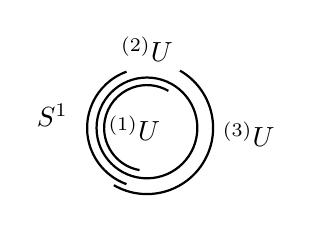
\begin{tikzpicture}[scale=0.8]
  \draw[thick] (0,0) circle (0.8);
  \draw[thick] (110:0.95) arc (110:250:0.95);
  \draw[thick] (60:1.05) arc (60:-120:1.05);
  \draw[thick] (-100:0.68) arc (-100:-300:0.68);
  \node[left] at (-1.1,0.2) {$S^1$};
  \node at (0,1.25) {${}^{(2)}U$};
  \node at (-0.2,0) {${}^{(1)}U$};
  \node[right] at (1.05,-0.1) {${}^{(3)}U$};
\end{tikzpicture}
\end{minipage}
\begin{minipage}[t]{0.36\textwidth}
neexistuje gl.\ nedeg.\ řez

\medskip
zvolme 3 okolí ${}^{(\alpha)}U$ \\
na každém (jednotkovou) bázi v lineárním bandle
\end{minipage}

\begin{center}
\begin{tikzpicture}[scale=0.55,>=Stealth]
  % triviální: 3 panely
  \foreach \i/\x/\a/\b in {1/0/200/340, 2/3.2/20/160, 3/6.4/250/290} {
    \begin{scope}[xshift=\x cm]
      \node at (-0.7,2) {${}^{(\i)}E$};
      \pic at (0,0) {gmIctyrAvalec};
      \foreach \t in {\a,...,\b} {}
      \foreach \t in {0,0.2,...,1} {
        \pgfmathsetmacro\ang{\a+\t*(\b-\a)}
        \draw[->,thick] ({0.8*cos(\ang)},{0.3+0.25*sin(\ang)}) -- ++(0,0.45);
      }
      \draw (0,-1.5) ellipse (0.8 and 0.22);
      \draw[very thick] ({0.8*cos(\a)},{-1.5+0.22*sin(\a)}) arc (\a:\b:0.8 and 0.22);
      \node at (0.9,-2.0) {${}^{(\i)}U$};
    \end{scope}
  }
  % twistovaný: 3 panely
  \foreach \i/\x/\a/\b/\s in {1/10.5/200/340/1, 2/13.7/20/160/1, 3/16.9/250/330/-1} {
    \begin{scope}[xshift=\x cm]
      \node at (-0.7,2) {${}^{(\i)}E$};
      \pic at (0,0) {gmIctyrAmobius};
      \foreach \t in {0,0.2,...,1} {
        \pgfmathsetmacro\ang{\a+\t*(\b-\a)}
        \draw[->,thick] ({0.75*cos(\ang)},{0.3+0.22*sin(\ang)}) -- ++(0,0.45*\s);
      }
      \draw (0,-1.5) ellipse (0.8 and 0.22);
      \draw[very thick] ({0.8*cos(\a)},{-1.5+0.22*sin(\a)}) arc (\a:\b:0.8 and 0.22);
      \node at (0.9,-2.0) {${}^{(\i)}U$};
    \end{scope}
  }
\end{tikzpicture}
\end{center}

\begin{minipage}{0.48\textwidth}
\begin{align*}
  {}^{(12)}\Phi &= [1] \\
  {}^{(23)}\Phi &= [1] \\
  {}^{(31)}\Phi &= [1]
\end{align*}
\end{minipage}
\begin{minipage}{0.48\textwidth}
\begin{align*}
  {}^{(12)}\Phi &= [1] \\
  \oprava{{}^{(23)}\Phi}{{}^{(21)}\Phi} &= [1] \\
  {}^{(31)}\Phi &= \vzorec{[-1]}
\end{align*}
\end{minipage}
\end{priklad}

\begin{vysvetleni}[Proč je Möbiův bandl netriviální]
Kružnici pokryjeme třemi oblouky ${}^{(1)}U,{}^{(2)}U,{}^{(3)}U$, které se překrývají po dvou ($12$, $23$, $31$); trojný průnik je prázdný, takže
kocyklus nic neomezuje a přechodová \uv{matice} $1\times1$ je na každém překryvu jen číslo $\neq0$.
(Proto jsou potřeba právě ${}^{(12)}\Phi,{}^{(23)}\Phi,{}^{(31)}\Phi$; ${}^{(21)}\Phi={}^{(12)}\Phi^{-1}$ by nic nového neříkalo.)
Při změně bází ${}^{(\alpha)}\mu$ (spojité nenulové funkce na souvislém ${}^{(\alpha)}U$, tedy s konstantním znaménkem) se znaménko součinu
${}^{(12)}\Phi\,{}^{(23)}\Phi\,{}^{(31)}\Phi$ nemění -- znaménka faktorů $\mu$ se vykrátí. Součin $>0$ dává válec (triviální bandl), $<0$ Möbiův pásek: obejdeme-li kružnici, báze se překlopí,
a proto neexistuje všude nenulový spojitý řez. Znaménko součinu je tzv.\ první Stiefelova--Whitneyova třída (orientovatelnost bandlu).
\end{vysvetleni}

%----------------------------------------------------------------------
\newpage
\strana{GMI-04a-8}
\tikzset{
  pics/gmIctyrAtorus/.style={code={%
    % vnější obrys rozříznutého torusu
    \draw[thick] (-0.75,-1.05) .. controls (-2.4,-0.9) and (-2.5,1.6) .. (0,1.65)
                 .. controls (2.5,1.6) and (2.4,-0.9) .. (0.75,-1.05);
    % vnitřní díra
    \draw (-1.1,0.15) .. controls (-0.9,0.7) and (0.9,0.7) .. (1.1,0.15);
    \draw (-0.9,0.35) .. controls (-0.6,-0.05) and (0.6,-0.05) .. (0.9,0.35);
    % vlákno P_y M nahoře
    \draw (0.25,1.62) .. controls (0.05,1.3) and (0.05,0.85) .. (0.3,0.62);
    \draw[dashed] (0.25,1.62) .. controls (0.5,1.3) and (0.5,0.85) .. (0.3,0.62);
    \node at (0,1.35) {\scriptsize $\mathbb{P}_yM$};
    % dvě vlákna P_x M v řezu
    \draw (-0.75,-0.25) ellipse (0.18 and 0.8);
    \draw (0.75,-0.25) ellipse (0.18 and 0.8);
  }}
}

\begin{priklad}[Př: příklad netriviálního nevektorového bandlu -- torus $T$ vs.\ Kleinova láhev $K$]
\begin{tabular}{ll}
$M = S^1$ & podkladová varieta \\
$\mathbb{P} = S^1$ & standardní fiber
\end{tabular}

\begin{center}
\begin{tikzpicture}[>=Stealth,scale=0.95]
  % torus
  \pic at (0,0) {gmIctyrAtorus};
  \draw[<->] (-0.6,0.15) -- (0.6,0.15);
  \draw[<->] (-0.6,-0.25) -- (0.6,-0.25);
  \draw[<->] (-0.6,-0.65) -- (0.6,-0.65);
  \node at (-2.3,-1.0) {$T\equiv\mathbb{P}M$};
  \node at (-0.8,-1.35) {\small $\mathbb{P}_xM$};
  \node at (0.8,-1.35) {\small $\mathbb{P}_xM$};
  \draw (0,-2.9) ellipse (1.7 and 0.8);
  \fill (-0.35,-3.7) circle (1.5pt) (0.35,-3.7) circle (1.5pt) (0,-2.1) circle (1.5pt);
  \draw[<->] (-0.3,-3.7) -- (0.3,-3.7);
  \node[below] at (-0.35,-3.7) {$x$}; \node[below] at (0.35,-3.7) {$x$};
  \node[below] at (0,-2.15) {$y$};
  \node at (1.95,-3.4) {$M$};
  \node at (0,-4.4) {torus};
  % standardní fibr
  \draw[thick] (4,0.2) circle (0.7);
  \node at (4,-0.95) {$\mathbb{P} = S^1$};
  % Kleinova láhev
  \begin{scope}[xshift=8cm]
    \pic at (0,0) {gmIctyrAtorus};
    \draw[<->] (-0.6,0.3) -- (0.6,-0.8);
    \draw[<->] (-0.6,-0.8) -- (0.6,0.3);
    \draw[<->] (-0.6,-0.25) -- (0.6,-0.25);
    \node at (2.3,-1.0) {$K\equiv\mathbb{P}M$};
    \node at (-0.8,-1.35) {\small $\mathbb{P}_xM$};
    \node at (0.8,-1.35) {\small $\mathbb{P}_xM$};
    \draw (0,-2.9) ellipse (1.7 and 0.8);
    \fill (-0.35,-3.7) circle (1.5pt) (0.35,-3.7) circle (1.5pt) (0,-2.1) circle (1.5pt);
    \draw[<->] (-0.3,-3.7) -- (0.3,-3.7);
    \node[below] at (-0.35,-3.7) {$x$}; \node[below] at (0.35,-3.7) {$x$};
    \node[below] at (0,-2.15) {$y$};
    \node at (1.95,-3.4) {$M$};
    \node at (0,-4.4) {Kleinova láhev};
  \end{scope}
\end{tikzpicture}
\end{center}

$M = S^1$ se získá periodickým ztotožněním intervalu $I$ \\
$\mathbb{P}M$ se získá vhodným ztotožněním fibrů $S^1$ na krajích intervalu $I$ z přímého součinu $I\times S^1$ \\
dvě možnosti ztotožnění -- \kw{přímé} a \oprava{\kw{zrcadlové} (reflexí)}{antipodální}
\end{priklad}

\begin{vysvetleni}[Torus vs.\ Kleinova láhev jako bandly]
Oba prostory jsou bandly nad $S^1$ s vláknem $S^1$: vezmeme válec $I\times S^1$ a slepíme kruhové konce pomocí zobrazení $f:S^1\to S^1$.
Pro $f=\mathrm{id}$ (přímé ztotožnění) vznikne torus $S^1\times S^1$ (triviální bandl), pro $f$ = zrcadlení kružnice (mění orientaci, jak ukazují
zkřížené šipky v obrázku) vznikne Kleinova láhev. Antipodální zobrazení kružnice je rotace o $\pi$, která je spojitě deformovatelná na identitu,
a dala by proto opět torus -- odtud oprava výše. Přechodová zobrazení tu nejsou lineární, leží v $\mathrm{Aut}\,\mathbb{E}=\mathrm{Diff}(S^1)$;
jde o \uv{nevektorový} bandl. Kleinova láhev je neorientovatelná, a proto není homeomorfní toru.
\end{vysvetleni}

\begin{priklad}[Př]
stejná situace je pro libovolnou sféru $S^n$ nad $S^1$ \\
\quad $M = S^1$ \\
\quad $\mathbb{P} = S^n$ \\
$\mathbb{P}M$ buď sférický tórus nebo zobecněná Kleinova láhev
\end{priklad}

\begin{vysvetleni}[Bandly $S^n$ nad $S^1$]
Bandl nad $S^1$ je určen jediným \uv{slepovacím} zobrazením $f:S^n\to S^n$ až na spojitou deformaci; difeomorfismy $S^n$ mají dvě třídy -- zachovávající
a měnící orientaci. Zachovávající dávají $S^1\times S^n$, měnící (např.\ zrcadlení jedné souřadnice) zobecněnou Kleinovu láhev.
Pozor: antipodální zobrazení $S^n$ mění orientaci jen pro sudé $n$ (stupeň $(-1)^{n+1}$), proto je obecně správné mluvit o zrcadlení.
\end{vysvetleni}

%----------------------------------------------------------------------
\newpage
\strana{GMI-04a-9}
\begin{priklad}[Př: Hopfova fibrace]
\begin{tabular}{lll}
$M = S^2$ & & podkladová varieta \\
$\mathbb{P} = S^1$ & & standardní fiber \\
$\mathbb{H} = \mathbb{P}M = S^3$ & & totální bandl
\end{tabular}

\medskip
$\mathbb{H} = S^3$ \quad v 4D souřadnicích $(a,b,c,d)$ \qquad $a^2 + b^2 + c^2 + d^2 = 1$ \\
$M = S^2$ \quad v 3D souřadnicích $(x,y,z)$ \qquad $x^2 + y^2 + z^2 = 1$

projekce \quad $\pi:\mathbb{H}\to M$
\[
  \vzorec{\pi(a,b,c,d) = \big(a^2 + b^2 - c^2 - d^2,\ 2(ad + bc),\ 2(bd - ac)\big)}
\]
fiber nad $x = \pi(a,b,c,d)$ \\
\quad dán rotací $(a,b,c,d)$ v rovinách $ab$ a $cd$ o úhel $\theta$
\[
  \begin{aligned}
  R_\theta(a,b,c,d) = \big(&a\cos\theta - b\sin\theta,\ b\cos\theta + a\sin\theta,\\
     &\oprava{c\cos\theta + d\sin\theta}{c\cos\theta - d\sin\theta},\\
     &\oprava{d\cos\theta - c\sin\theta}{d\cos\theta + c\sin\theta}\big)
  \end{aligned}
\]
\quad to vytváří kružnici se stejnou projekcí \\
\quad\quad $\pi R_\theta(a,b,c,d) = x$
\end{priklad}

\begin{vysvetleni}[Hopfova fibrace v komplexních souřadnicích]
Označme $z_1=a+\mathrm{i}b$, $z_2=c+\mathrm{i}d$, takže $S^3=\{|z_1|^2+|z_2|^2=1\}\subset\mathbb{C}^2$. Projekce z poznámek je
$\pi=\big(|z_1|^2-|z_2|^2,\ 2\,\mathrm{Im}(z_1z_2),\ -2\,\mathrm{Re}(z_1z_2)\big)$; snadno $|\pi|^2=(|z_1|^2+|z_2|^2)^2=1$.
Je invariantní vůči $(z_1,z_2)\mapsto(e^{\mathrm{i}\theta}z_1,e^{-\mathrm{i}\theta}z_2)$ -- tj.\ rotace v rovině $cd$ musí jít \emph{opačným} směrem než v rovině $ab$.
S rotací v originále ($z_2\mapsto e^{\mathrm{i}\theta}z_2$) by se $z_1z_2$ násobilo $e^{2\mathrm{i}\theta}$ a projekce by se měnila
(např.\ bod $(\tfrac{1}{\sqrt2},0,\tfrac{1}{\sqrt2},0)$ s $\pi=(0,0,-1)$ by se pro $\theta=\pi/2$ dostal do bodu s $\pi=(0,0,1)$); odtud oprava znamének.
Vlákna jsou kružnice (každé dvě jsou spolu propletené) a bandl je netriviální: $S^3\not\cong S^2\times S^1$ (např.\ $S^3$ je jednoduše souvislá).
Jde o základní příklad hlavního $U(1)$-bandlu (souvisí s Diracovým monopólem).
\end{vysvetleni}

